\chapter{IDE}
An integrated development environment (IDE) or interactive development environment is a software, typically consisting of a graphical user interface, a code editor and a compiler. The main purpose of IDEs is to make programming for the developer as easy as possible, offering functions like syntax-highlighting, auto-complete and source-generation. The following sub-chapters describe which IDEs had been used in the project.     

%George, Pokorny
\section{Andorid SDK Eclipse}

Eclipse is an integrated development environment (IDE) mostly written in Java developed by the Eclipse Foundation, founded my IBM.

Eclipse can be used as development environment for almost every common programming language such as Java C++ or Python. 

\subsection{Eclipse Workbench}
The Eclipse GUI contains four different sections as one can see in the figure bellow
\\ 
\begin{figure}[h]
\centering
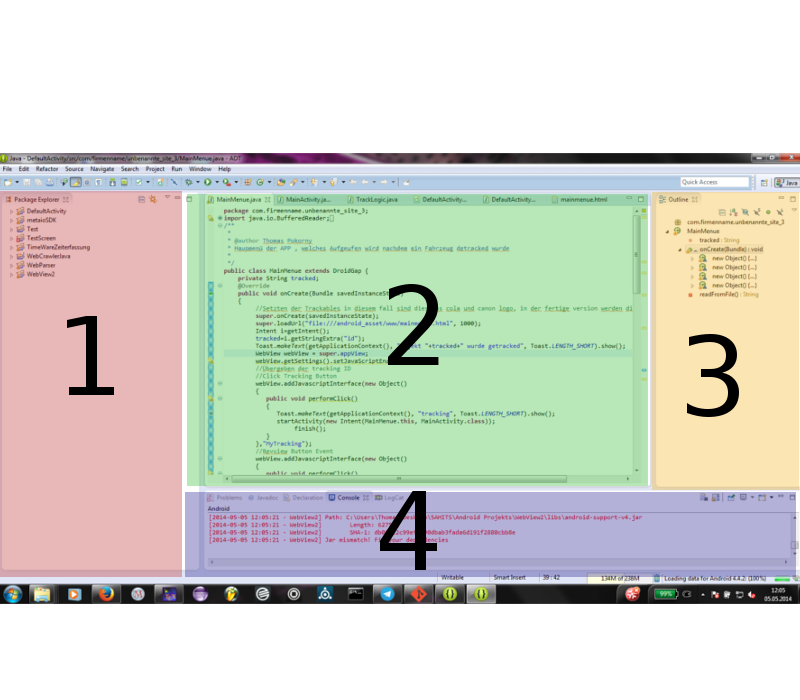
\includegraphics[width=400pt,height=350pt,keepaspectratio]{graphics/eclipse.png}
\caption{Eclipse Workbench}
\end{figure}

\begin{enumerate}
\item Overview of all Project inside the workspace
\item Text-editor with functions like: syntax-highlighting, auto-complete, source-generation.
\item The outline contains attributes, methods and classes of the selected file inside the editor. 
\item The last sections shows the console-output     
\end{enumerate}

\subsection{Android SDK}
Their is an Android ADT (Adnroid Development Tools) plug-in available for Eclipse. ADT makes it easy to set up new Android projects, create an application UI, add packages based on the Android Framework API, debug applications using the Android SDK tools, and export signed .apk files in order to distribute  applications.














%Korabach
\section{JetBrains WebStorm}
The applications logic had to be created with a programming language called JavaScript. Because of that, the project group had to find a development environment that's best suited for this language. JetBrains WebStorm 7.0.3 was best fit for all future tasks and should be the environment in which JavaScript had been developed. 
\\

However, not only JavaScript, but also HTML as well as CSS could be developed with this IDE. All information about this product can be found on Jet Brains homepage.\cite{webstorm}
\subsection{Overview}
\textit{''JetBrains WebStorm is a professional JavaScript IDE that supports a wide range of modern technologies related to JavaScript programming language, HTML and  CSS, and provides the complete experience for productive Web development.''}\cite{webstorm}
\\

\textit{''WebStorm offers developers an intelligent code editor that truly supports the structure of code written in JavaScript, HTML or CSS, as well as their modern  successors. It features the best-of-breed coding assistance for a whole set of  cutting-edge web technologies, including code completion, refactorings, code formatting, on-the-fly error prevention, and much more.''}\cite{webstorm}
\\

\textit{''WebStorm is also great for developing Node.js applications. Together with integrated instruments 
for testing, debugging and code analysis and integration with various VCS, WebStorm is an essential tool for powerful and productive web development.''}\cite{webstorm}
\\

\begin{figure}[h]
\centering
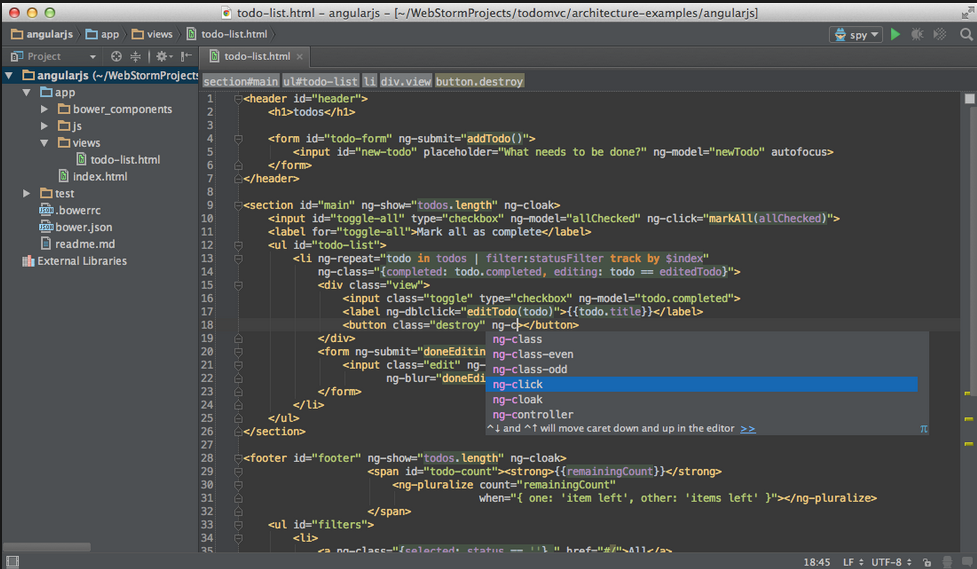
\includegraphics[width=1\linewidth]{graphics/chapter3/1}
\caption{WebStorm Interface}
\end{figure}


\subsection{Features}
\begin{itemize}
\item \textit{Intelligent JavaScript, HTML, and CSS editor with syntax highlighting, code completion, configurable formatting configuration, refactorings, on-the-fly error detection and support of language mixtures.}\cite{webstorm}
\item \textit{Support for a wide range of technologies: TypeScript, CoffeeScript, Dart, LESS, Sass, Stylus, Compass, EJS, Handlebars, Mustache, Web Components, Jade, Emmet, and many more.
\item Productivity-boosting Live Edit feature: See the changes in the browser immediately without reloading the page.}\cite{webstorm}
\item 
\textit{JavaScript debugger for Chrome and Firefox, with breakpoints, stepping, frames view and watchers. Full-featured debugging of TypeScript, CoffeeScript and Dart with sourcemaps.}\cite{webstorm}
\item 
\textit{File Watchers for automatic compilation/transpilation of higher-level languages like TypeScript, CoffeeScript, LESS, Sass, and Stylus.}\cite{webstorm}
\item 
\textit{A debugger for Node.js applications with the latest features of V8 Debugger Protocol.}\cite{webstorm}
\item 
\textit{Intelligent code inspections, one-click quick-fix suggestions, JSHint, JSLint, and Google Closure Linter.}\cite{webstorm}
\item
\textit{JavaScript unit testing with integrated JSTestDriver or Karma test runner with code coverage.}\cite{webstorm}
\end{itemize}
















%Fegerl
\section{Visual Studio}
Visual Studio is a development environment for creating applications for Microsoft platforms and beyond. It provides the programming languages C++, C\#, HTML and JavaScript.
The newest available version of Visual Studio is Visual Studio 2013.\cite{vstudio1}

\begin{figure}[htbp]
\centering
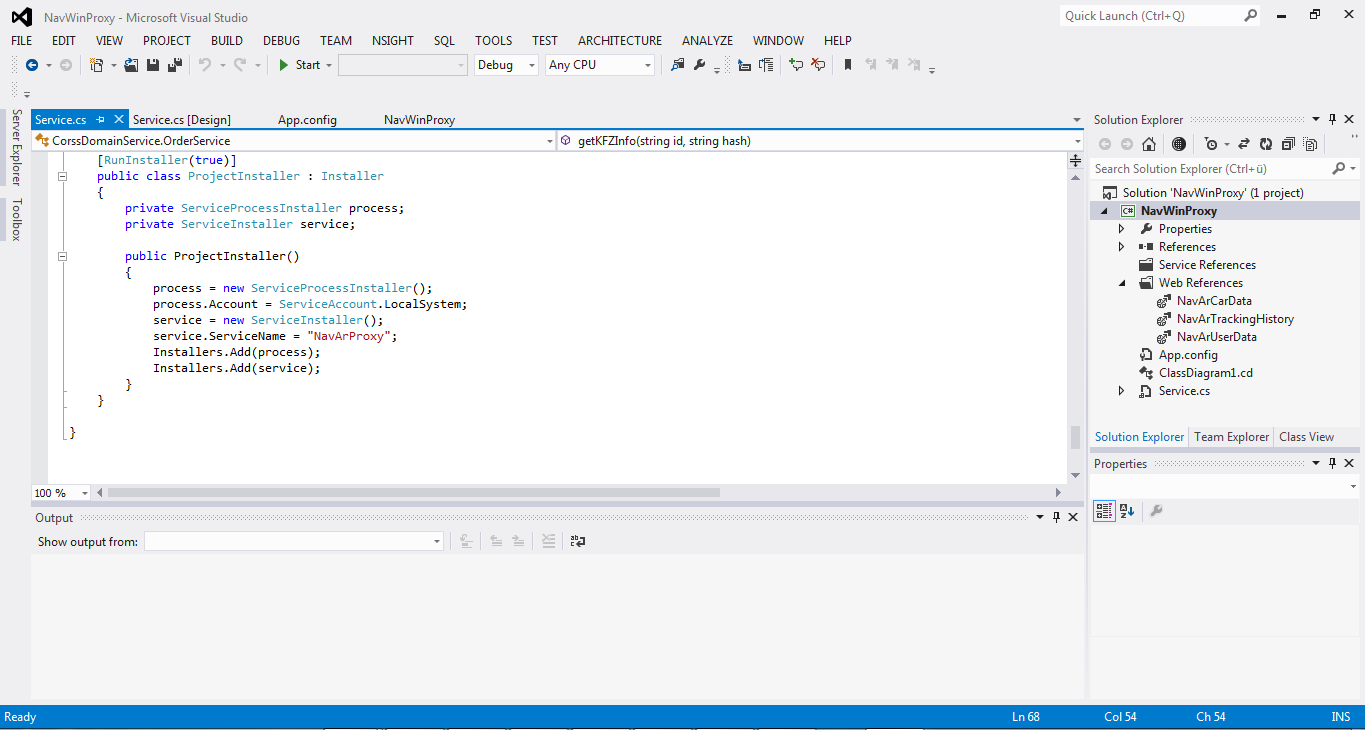
\includegraphics[width=140mm,height=150mm,keepaspectratio]{graphics/visualstudio.PNG}
\caption{Visualstudio development environment\cite{ajax}}
\end{figure}


\subsection{Visual Studio 2013}
Visual Studio 2013 provides four commercial versions: Ultimate, Premium,Pro and Test Pro. The difference between these versions can be found on the official Visual Studio page : http://www.visualstudio.com/products/compare-visual-
\\
studio-products-vs
\newpage
